\chapter{Introducción Específica}\label{Chapter2}

El capítulo presenta en detalle los temas aplicados en el desarrollo del trabajo y
las definiciones realizadas en el inicio del proyecto. Permite conocer los requisitos
y herramientas planteados.

\section{Requerimientos y supuestos}

  En el contexto del desarrollo de proyectos tecnológicos en el ámbito empresarial,
  es común enfrentarse a la necesidad de optimizar recursos, tanto económicos como
  técnicos. Un escenario particularmente desafiante se presenta cuando se
  identifica la oportunidad de reemplazar componentes de terceros, que suelen
  incurrir en costos de licencia significativos, por soluciones propias que no
  solo reduzcan costos sino que también ofrezcan la posibilidad de adaptación y
  mejora continua según las necesidades específicas del proyecto. Este fue
  precisamente el escenario en el que se enmarcó el desarrollo del módulo
  mientras trabajaba en la empresa VideoSwitch.

  La iniciativa para desarrollar un módulo SDI propio surgió como respuesta a la
  necesidad de contar con una solución más flexible y económicamente viable que
  los \textit{IP cores} de la empresa Altera que se estaban utilizando. Estos
  últimos, aunque funcionales, imponían limitaciones tanto en términos de costos
  como de adaptabilidad a los constantes cambios de versión de las herramientas
  de desarrollo y a la posibilidad de usar dispositivos de otras marcas, en un
  mercado con grandes problemas de abastecimiento. En este sentido, el desarrollo
  de un módulo propio se presentó no solo como una oportunidad de ahorro económico
  sino también como un desafío técnico que permitiría al equipo de
  desarrollo profundizar en el conocimiento y manejo de las interfaces de alta
  velocidad, además de ejercer un control total sobre las características y
  rendimiento del módulo.

  Para abordar este trabajo, fue necesario realizar un análisis exhaustivo de
  los requisitos técnicos y las expectativas de rendimiento que debería cumplir
  el módulo SDI\@. Este análisis implicó un trabajo colaborativo entre los
  equipos de \textit{software} y \textit{hardware} de la empresa.

  El proceso de definición de requerimientos se enfocó en capturar las
  necesidades reales de los proyectos actuales y futuros, considerando tanto
  las limitaciones técnicas inherentes al \textit{hardware} disponible como las
  oportunidades de innovación. Este enfoque permitió establecer una hoja de ruta
  clara para el desarrollo del módulo, priorizando aquellos aspectos críticos
  para el rendimiento y la funcionalidad, sin perder de vista la flexibilidad.
  Así es cómo se llegó a la siguiente lista de requerimientos.

  \begin{enumerate}
      \item Verificación
      \begin{enumerate}
          \item \textit{Tests} unitarios de cada módulo funcional.
          \item Simulación de bloques de protocolo completos.
          \item Simulación del sistema completo haciendo \textit{loopback} entre el trasmisor y el receptor.
      \end{enumerate}
      % \item Validación
      % \begin{enumerate}
      %     \item Medición y observación de audio y video luego de pasar por el sistema completo.
      %     \item Medición de los los paquetes con un analizador según la norma.
      %     \item Cumplir con el bitrate de los estándares dentro del rango de SD-SDI y 3G-SDI.
      % \end{enumerate}
      \item Funcionalidad
      \begin{enumerate}
          \item Obtener las tasas de datos contempladas dentro del rango de las normas SD-SDI y 3G-SDI\@.
          \item Obtener un diseño sin problemas de \textit{timing} en las señales entre dominios de reloj
          dentro del módulo.
          \item Obtener un módulo sin problemas de \textit{timing} por \textit{setup} o \textit{hold} en las señales de entrada y salida.
          \item La implementación del sistema no debe ocupar más de 3000 \textit{Logic Array Blocks} en la FPGA\@.
      \end{enumerate}
      \item Metodología de trabajo
      \begin{enumerate}
          \item Control de versiones mediante SVN o Git.
          \item Desarrollo en Quartus con licencias para análisis de \textit{timing} y simulaciones o herramientas \textit{open source}.
          \item Planificación y documentación mediante Redmine o Gitlab.
          \item Diseño modular.
      \end{enumerate}
      \item Documentación
      \begin{enumerate}
          \item Confección de la memoria técnica.
          \item Confección de documentación del diseño del módulo.
          \item Confección de documentación de uso del módulo.
      \end{enumerate}
  \end{enumerate}

  Sin embargo, como suele ocurrir en el dinámico entorno empresarial, los cambios
  en las prioridades de gestión y mi posterior salida de la empresa llevaron a que
  casi ninguno de los supuestos planteados inicialmente para el desarrollo del
  módulo se cumpliera. Estas modificaciones en el enfoque y la asignación de
  recursos afectaron directamente la ejecución y el avance del proyecto, limitando
  la capacidad para alcanzar los objetivos propuestos con la rapidez y eficacia
  esperadas.

  A continuación, se listan los supuestos originales bajo los cuales se había
  concebido el proyecto, resaltando que, desafortunadamente, solo el último de
  estos se cumplió:

  \begin{enumerate}
      \item Se cuenta con el hardware necesario para su implementación, con driver SDI y una FPGA Cyclone V con hard-transceivers.
      \item Se cuenta con los instrumentos de medición necesarios.
      \item Se cuenta con las licencias de software necesarias para el desarrollo.
      \item Se cuenta con el módulo que se desea remplazar.
      \item Se cuenta con el tiempo necesario dentro de la empresa para hacer el desarrollo y las pruebas.
      \item Se cuenta con las normas en cuestión.
  \end{enumerate}

  El único supuesto que se logró cumplir fue el acceso a las normas pertinentes
  al desarrollo del módulo. Este item, aunque significativo para el entendimiento
  y la conceptualización del proyecto, resultó insuficiente para poder cumplir
  con los objetivos y plazos planteados originalmente.
  
  % contrarrestar las
  % limitaciones impuestas por la no concreción de los otros supuestos necesarios
  % para un desarrollo y ejecución exitosos del módulo SDI\@.

  Esta situación refleja los retos que enfrentan los proyectos de innovación
  tecnológica en el ámbito empresarial, donde las fluctuaciones en las prioridades
  organizacionales y los cambios en los equipos de trabajo pueden alterar
  significativamente la trayectoria y los resultados de iniciativas críticas,
  subrayando la importancia de una gestión flexible y adaptativa frente a las
  inevitables dinámicas del entorno empresarial.

  Por todas estas razones, en el diseño final se decidió apostar por el uso de
  herramientas de código abierto y evitar la dependencia de hardware específico y
  propietario. Esta decisión estratégica buscaba mitigar los riesgos asociados a
  las limitaciones de \textit{hardware} y \textit{software}, permitiendo una
  mayor flexibilidad y adaptabilidad frente a los cambios y desafíos del entorno.

  El compromiso con soluciones de código abierto no solo facilita la gestión de
  recursos y la independencia tecnológica, sino que también promueve una cultura
  de innovación y colaboración, esenciales para el desarrollo sostenible del
  proyecto en un contexto de incertidumbre y cambio constante.

\section{Nociones básicas del sistema}

  \subsection{Formato de datos}

  En aplicaciones SD y ED, el formato de datos serie se define con un ancho de 10 bits,
  mientras que en aplicaciones HD es de 20 bits, divididos en dos flujos de datos paralelos
  de 10 bits cada uno (conocidos como Y y C). El flujo de datos SD se organiza de la
  siguiente manera:

  \begin{verbatim}
  Cb Y Cr Y' Cb Y Cr Y'
  \end{verbatim}

  Mientras que los flujos de datos HD se organizan así:

  \begin{verbatim}
  Y
  Y Y' Y Y' Y Y' Y Y'
  C
  Cb Cr Cb Cr Cb Cr Cb Cr
  \end{verbatim}

  Para todas las interfaces digitales serie (excluyendo las codificaciones compuestas
  obsoletas), la codificación de color nativa es el formato YCbCr 4:2:2. El canal de
  luminancia (Y) se codifica con un ancho de banda completo (13,5 MHz en SD de 270 Mbit/s,
  ~75 MHz en HD), y los dos canales de crominancia (Cb y Cr) se submuestrean horizontalmente
  y se codifican con la mitad de ancho de banda (6.75 MHz o 37.5 MHz). Las muestras Y, Cr y
  Cb están co-situadas (adquiridas en el mismo instante de tiempo), y la muestra Y' se
  adquiere en el momento intermedio entre dos muestras Y adyacentes.

  En lo anterior, Y se refiere a muestras de luminancia, y C a muestras de crominancia. Cr y
  Cb se refieren además a los canales de diferencia de color rojo y azul; ver vídeo por
  componentes para más información. Esta sección solo discute la codificación de color nativa
  de SDI\@; otras codificaciones de color son posibles tratando la interfaz como un canal de
  datos de 10 bits genérico. El uso de otras codificaciones de colorimetría, y la conversión
  a y desde el espacio de color RGB, se discute a continuación.

  La carga útil de vídeo (así como la carga útil de datos auxiliares) puede usar cualquier
  palabra de 10 bits en el rango de 4 a 1,019 (004\textsubscript{16} a 3FB\textsubscript{16})
  inclusive; los valores 0–3 y 1,020–1,023 (3FC\textsubscript{16}–3FF\textsubscript{16}) están
  reservados y no pueden aparecer en ninguna parte de la carga útil. Estas palabras reservadas
  tienen dos propósitos; se utilizan tanto para paquetes de sincronización como para cabeceras
  de datos auxiliares.

  \subsection{Paquetes de sincronización}

  Un paquete de sincronización (comúnmente conocido como la señal de referencia de tiempo o TRS)
  ocurre inmediatamente antes de la primera muestra activa en cada línea, e inmediatamente después
  de la última muestra activa (y antes del inicio de la región de borrado horizontal). El paquete
  de sincronización consta de cuatro palabras de 10 bits, las primeras tres palabras siempre son
  las mismas: 3FF\textsubscript{16}, 0, 0; la cuarta consta de 3 bits de bandera, junto con un código de corrección
  de errores. Como resultado, hay 8 paquetes de sincronización diferentes posibles.

  En las interfaces HD-SDI y de enlace dual, los paquetes de sincronización deben ocurrir
  simultáneamente en ambos flujos de datos Y y C. (Se permite cierto retraso entre los dos cables
  en una interfaz de enlace dual; se espera que el equipo que soporta enlace dual almacene en
  búfer el enlace líder para permitir que el otro enlace se ponga al día). En interfaces SD-SDI y
  de definición mejorada, solo hay un flujo de datos, y por lo tanto, solo un paquete de
  sincronización a la vez. Aparte del tema de cuántos paquetes aparecen, su formato es el mismo en
  todas las versiones de la interfaz digital-serial.

  Los bits de bandera encontrados en la cuarta palabra (comúnmente conocida como la palabra XYZ)
  son conocidos como H, F y V. El bit H indica el inicio del borrado horizontal; y los bits de
  sincronización que preceden inmediatamente a la región de borrado horizontal deben tener H
  establecido en uno. Tales paquetes se conocen comúnmente como paquetes de Fin de Vídeo Activo, o
  paquetes EAV\@. De manera similar, el paquete que aparece inmediatamente antes del inicio del vídeo
  activo tiene H establecido en 0; este es el paquete de Inicio de Vídeo Activo o paquete SAV\@.

  De manera similar, el bit V se utiliza para indicar el inicio de la región de borrado vertical; un
  paquete EAV con V=1 indica que la siguiente línea (las líneas se consideran que comienzan con el
  paquete SAV) será la primera línea del borrado vertical. De manera similar, un paquete SAV con V=1
  indica que la línea actual es la primera línea del vídeo activo después del borrado vertical. Los
  paquetes SAV/EAV con V=0 indican líneas dentro de la región de vídeo activo, o dentro de la región
  de borrado horizontal, pero no el inicio o el final de ninguna de estas regiones.

  El bit F se utiliza para distinguir entre campos en formatos entrelazados o segmentados
  progresivamente. En formatos progresivos, F siempre es 0. En formatos entrelazados o segmentados
  progresivamente, F es 0 para todas las líneas en el primer campo o segmento, y 1 para todas las
  líneas en el segundo campo o segmento. (La designación de cuál de los dos campos o segmentos se
  considera el primero es arbitraria).

\section{Estructura general del sistema y diagrama en bloques}

  En cuanto a la implementación en FPGA, la interfaz SDI consta de dos capas
  independientes, que se pueden visualizar en la figura~\ref{fig:sdi1}, la de
  recepción/transmisión y la de protocolo, por tal motivo el módulo deberá
  implementar ambas instancias de manera separada. Para la primera, se suelen
  usar \textit{hard-transceivers}, contenidos en la FPGA o \textit{soft-transceivers}
  instanciados en la lógica programable, para las aplicaciones con menor demanda
  de tasa de datos. Este módulo se puede encargar de muestrear la entrada
  asincrónica, sincronizarse a la misma y deserializar los datos, para casos más
  exigentes es necesario usar un \textit{hard-transceivers}. En este diseño no se
  pretende resolver esta parte del desarrollo, sino usar las soluciones que
  proporcionan los fabricantes de los dispositivos, que por lo general son de uso
  libre, aunque propietarias. El desarrollo que puede ser necesario dependiendo
  el fabricante que se elija es el controlador de dicho módulo.

  Para la segunda etapa, se debe implementar un submódulo que trabaje en el dominio
  de los datos paralelizados y tenga la información propia del protocolo para
  interpretar, acondicionar y validar la señal. Esta parte del desarrollo se
  encarga principalmente de la sincronización de paquetes y de la detección de
  errores. Aunque la interfaz funciona en un solo sentido a la vez, debe ser
  configurable para funcionar como transmisor y receptor de manera separada, como
  se ilustra en la figura~\ref{fig:sdi1}. Por lo tanto, el módulo debe ser capaz
  de tomar la señal serie que llega a la FPGA desde el \textit{driver} del cable,
  deserializarla y procesarla en un sentido y empaquetarla (acorde al
  protocolo) y serializarla en el otro sentido.

  \begin{figure}[htbp]
      \centering
      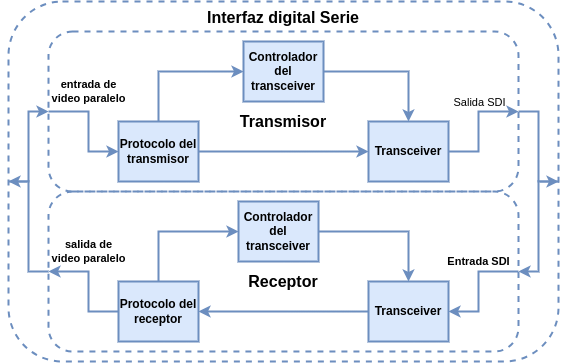
\includegraphics[width=\linewidth]{./Figures/sdi.png}
      \caption{Diagrama en bloques general de interfaz digital serie.}\label{fig:sdi1}
  \end{figure}

\section{Estándares soportados por la interfaz}

  El módulo soporta SMPTE SD/HD/3G-SDI implementa tres estándares de la interfaz:

  \begin{itemize}
      \item SD-SDI (SMPTE ST 259): señal digital de televisión estándar~\citep{st259}.
      \item HD-SDI (SMPTE ST 292\-1): interfaz serie de señal de 1,5 Gb/s~\citep{st292}.
      \item 3G-SDI (SMPTE ST 424): interfaz serie de señal de 3 Gb/s~\citep{st424}.
  \end{itemize}

  \subsection{Definición estándar}

  El módulo está diseñado para soportar la tasa de bits de 270 Mb/s y es compatible
  con el estándar de detección y manejo de errores o EDH (del inglés, \textit{Error
  Detection and Handling}) SMPTE RP 165~\citep{st165} para las secciones de
  recepción y transmisión~\citep{castr}.

  \subsection{Alta definición}

  Aunque el estándar se llama interfaz de 1,5 Gb/s, las tasas de bits admitidas
  por HD-SDI son en realidad de 1,485 Gb/s y 1,485/1,001 Gb/s. El módulo es
  compatible con ambas tasas de bits y con la generación (transmisor) y
  verificación (receptor) de valores CRC (del inglés, \textit{Cyclic Redundancy Check})
  para cada línea de video, así como la inserción (transmisor) y captura (receptor)
  de valores de número de línea para cada línea~\citep{castr}.

  \subsection{Ultra alta definición}

  Como con el estándar anterior, llama interfaz de 3 Gb/s, pero las tasas de bits
  real son de 2,97 Gb/s y 2,97/1,001 Gb/s. El módulo es compatible con ambas tasas
  de bits. 3G-SDI admite varios niveles de mapeo diferentes, descritos en el
  estándar SMPTE ST 425\-1. El núcleo es compatible con todos estos niveles. Al
  igual que con el estándar HD-SDI, el núcleo también es compatible con la
  generación y verificación de CRC, así como la inserción y captura de números de
  línea para 3G-SDI\@~\citep{castr}.

  \subsection{Identificación de carga útil y soporte de datos auxiliares}

  El módulo implementa una capacidad de inserción de paquetes de datos auxiliares
  de identificación de carga útil SMPTE ST 352~\citep{st352} para el transmisor que funciona en
  todos los 3 modos SDI ya mencionados. El lado receptor también detecta y captura
  los cuatro bytes de datos de los paquetes de identificación de carga útil ST 352.

  Además, implementa la inserción de paquetes de datos auxiliares antes de la
  transmisión. Aunque el módulo no proporciona una capacidad de inserción de paquetes
  de datos auxiliares, excepto para los paquetes de identificación de carga útil
  ST 352~\citep{st352}, tiene puertos de datos necesarios para permitir que la inserción de
  paquetes de datos auxiliares sea implementada por el usuario. En el lado del
  receptor, todos los datos auxiliares insertados son preservados por el receptor.
  El módulo pueden procesar el flujo de datos SDI recibidos y/o modificar los datos
  auxiliares según sea necesario~\citep{design}.

\section{Simulación y verificación}

  La verificación y validación de código y modelos por medio de simulación es
  un aspecto crucial para garantizar calidad y reducir tiempos de desarrollo,
  sobre todo en sistemas críticos. La verificación garantiza con simulaciones y
  permite la corrección del código, antes de hacer pruebas en el mundo real, que
  son más lentas y costosas. La validación se relaciona con la conexión del
  desarrollo con el mundo real y su uso previsto, implica contar con el
  \textit{hardware} y el instrumental de medición. Además, en sistemas de alta
  complejidad la simulación permite probar cada módulo por separado, técnica que
  facilita la integración y permite distinguir con claridad los errores, lo que
  acelera proceso de aprendizaje y comprensión del sistema. Por otro lado al ser
  capaces de simular datos de cierto modelo, se garantiza que uno entiende el
  modelo, sus restricciones y limitaciones~\citep{testbench}.

  \begin{figure}[htbp]
      \centering
      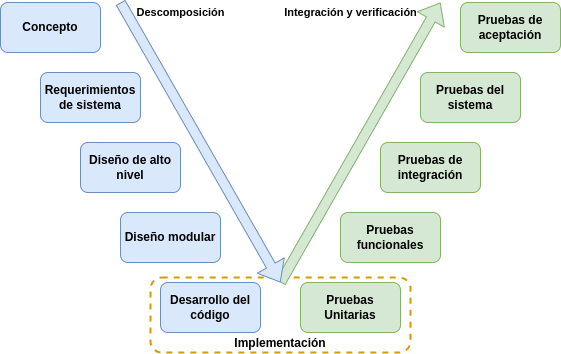
\includegraphics[width=\linewidth]{./Figures/verif.png}
      \caption{Diagrama pasos a seguir para diseñar, implementar y verificar un proyecto.}\label{fig:verif}
  \end{figure}

  % En este trabajo se llevaron a cabo test unitarios para cada módulo básico del
  % desarrollo e incluso aquellos que integraban varios submódulos, usando GHDL,
  % cocotb e integración continua en Github, pero para la verificación del sistema
  % completo fue necesario usar Quartus y ModelSim, ya que no se contaba con los
  % modelos de los Transceivers debido a que son herramientas propietarias.

  Las pruebas unitarias son a nivel de código y ayudan a eliminar
  problemas en una etapa temprana, principalmente el desarrollador es responsable
  de realizarla para su código.

  Las pruebas funcionales están asociadas con la fase de diseño de bajo nivel
  que garantiza que los módulos de códigos y unidades estén trabajando correctamente
  para ejecutar nuevas funciones o servicios.

  Las pruebas de integración están asociadas con la fase de diseño de alto
  nivel. Estas garantizan la integración entre todos los módulos del sistema después
  de agregar nuevas funciones o actualizaciones.

  Las pruebas de sistema están asociados con los requisitos y la fase de
  diseño del sistema. Combinan el \textit{software}, el \textit{hardware} y la
  integración de este sistema con otros sistemas externos.

  Las pruebas de aceptación del usuario están asociadas con la fase de
  análisis empresarial y operativo. Los usuarios clientes son los principales
  ejecutores de esta prueba basada en casos de prueba y escenarios que cubren los
  requisitos comerciales para garantizar que se haya entregado el producto correcto
  según las especificaciones.

  Dado que, durante la implementación de este desarrollo, no se disponía del
  equipamiento de la empresa VideoSwitch, se enfocó especialmente en las etapas
  iniciales. Se llevaron a cabo pruebas a nivel del sistema de manera parcial,
  omitiendo las pruebas de aceptación~\citep{testbench}.

  % Debido a que al momento de la ejecución de este desarrollo no se sigue contando
  % con el equipamiento de la empresa VideoSwitch, se puso especial énfasis en las
  % primeras etapas, ejecutando Las pruebas a nivel sistema solo de forma
  % parcial y dejando de lado Las pruebas de aceptación.

\section{Integración continua}

La integración continua o CI (del inglés, \textit{continuous integration}) es una
práctica que nace de la ingeniería de software, pero que en los últimos años se
a ido extendiendo a otras ramas de la ingeniería, que consiste en hacer
integraciones automáticas de un proyecto con cierta regularidad para así poder
detectar errores cuanto antes. Se entiende por integración la compilación o
síntesis y ejecución de pruebas de un proyecto completo y sus subsistemas. 

Por lo general se necesita un sistema de control de versiones que acompañe y
ejecute el proceso de CI\@. Los mismos también se complementan con otras
comprobaciones como las pruebas automatizadas de calidad del código, las
herramientas de revisión de estilo de sintaxis, entre otras.

Los beneficios comúnmente citados de la integración continua incluyen:
\begin{itemize}
  \item Detección temprana y mejorada de errores, y métricas que le permiten
  abordar los errores a tiempo, a veces tras solo unos minutos de la incorporación.
  \item Progreso continuo y demostrado para mejorar la retroalimentación.
  \item Mejor colaboración en equipo: todos los miembros del equipo pueden 
  cambiar el código, integrar el sistema y determinar rápidamente los conflictos
  con otras partes de este.
  \item Integración mejorada del sistema, lo que reduce las sorpresas al final
  del ciclo de vida del desarrollo.
  \item Menos cambios paralelos para la fusión y prueba.
  \item Reducción de cantidad de errores durante las pruebas del sistema.
  \item Sistemas actualizados constantemente en los que realizar las pruebas.
\end{itemize}

Para este trabajo se optó por usar Git como sistema de control de
versiones, más específicamente GitHub, que con GitHub Actions también entrega
la funcionalidad de integración continua~\citep{cicd}.